% Letters
% Letters are short reports of original research focused on an outstanding finding whose importance means that it will be of interest to scientists in other fields.

% They do not normally exceed 4 pages of Nature and, as a guideline, allow up to 30 references. They begin with a fully referenced paragraph, ideally of about 200 words, but certainly no more than 300 words, aimed at readers in other disciplines. This paragraph starts with a 2-3 sentence basic introduction to the field; followed by a one-sentence statement of the main conclusions starting 'Here we show' or equivalent phrase; and finally, 2-3 sentences putting the main findings into general context so it is clear how the results described in the paper have moved the field forwards.

% Please refer to our annotated example to see how the summary paragraph for a Letter should be constructed.

% The rest of the text is typically about 1,500 words long. Any discussion at the end of the text should be as succinct as possible, not repeating previous summary/introduction material, to briefly convey the general relevance of the work.

% Letters typically have 3 or 4 small display items (figures or tables).

% Word counts refer to the text of the paper. References, title, author list and acknowledgements do not have to be included in total word counts.

%%%%%%%%%%%%
% GAMEPLAN %
%%%%%%%%%%%%

%%%%%%%%%%%%%%%
%% MAIN TEXT %%
%%%%%%%%%%%%%%%

% introduction to the question of IA
% topography, climate, and lithology are important
% GEOCLIM model
% dependence on slope and lithology
% calibration (various feasible combinations of parameters)
% temperature and runoff from GFDL
% tested scenarios, including explanation of the paleoshoreline data
% IA is important, traps are less important
% limitations with approach
    % GFDL equilibrated by last 100 years?
    % not changing paleogeography
    % source term. Can cite: Rowan2016a related to spreading rate.
    % low resolution
    % GFDL model is quite old
    % kinetics are not changing between lithologies
    
%%%%%%%%%%%%%%%%%%%%%%%
%% MAIN TEXT FIGURES %%
%%%%%%%%%%%%%%%%%%%%%%%

% paleoshorelines
% steady state pCO2 for all scenarios

%%%%%%%%%%%%%%%%%%%%%%%%%%%%%%%
%% SUPPLEMENTARY INFORMATION %%
%%%%%%%%%%%%%%%%%%%%%%%%%%%%%%%

% details of DynSoil and GEOCLIM
% details of parameter exploration/calibration
    % basin data used for parameter exploration
% details of lithology implementation
    % including Sunda Shelf
% details of paleoshoreline reconstructions

%%%%%%%%%%%%%%%%%%%%%%%%%%%%%%%%%%%%%%
%% SUPPLMENTARY INFORMATION FIGURES %%
%%%%%%%%%%%%%%%%%%%%%%%%%%%%%%%%%%%%%%

% regolith model schematic
% maps of all scenarios

\documentclass[11pt,letterpaper]{article}

%\usepackage{fontspec}
%\usepackage[utf8]{inputenc}
\usepackage{textcomp,marvosym}
\usepackage{amsmath,amssymb}
\usepackage[normalem]{ulem}
\usepackage[left]{lineno}
\usepackage{booktabs}
\usepackage{changepage}
\usepackage{rotating}
\usepackage{color}
\usepackage{natbib}
\usepackage{setspace}
\usepackage{array}
\usepackage{fancyhdr}
\usepackage{graphicx}
\usepackage{xspace}
\usepackage[hidelinks]{hyperref}
\urlstyle{same}
\usepackage{threeparttable}
\doublespacing

\raggedright
\textwidth = 6.5 in
\textheight = 8.25 in
\oddsidemargin = 0.0 in
\evensidemargin = 0.0 in
\topmargin = 0.0 in
\headheight = 0.0 in
\headsep = 0.5 in
\parskip = 0.1 in
\parindent = 0.2in

% Bold the 'Figure #' in the caption and separate it from the title/caption with a period
% Captions will be left justified
\usepackage[aboveskip=1pt,labelfont=bf,labelsep=period,justification=raggedright,singlelinecheck=off]{caption}

% Remove brackets from numbering in List of References
%\makeatletter
%\renewcommand{\@biblabel}[1]{\quad#1.}
%\makeatother

% Self defined commands
\newcommand{\degreesC}{\textdegree C\xspace}
\newcommand{\degrees}{\textdegree\xspace}
\newcommand{\dC}{$\delta^{13}$C\xspace}
\newcommand{\dO}{$\delta^{18}$O\xspace}
\newcommand{\SrSr}{$^{87}$Sr/$^{86}$Sr\xspace}
\newcommand{\OsOs}{$^{187}$Os/$^{188}$Os\xspace}
\newcommand{\permil}{\textperthousand\xspace}
\newcommand{\UPb}{$^{206}$Pb/$^{238}$U\xspace}
\newcommand{\pCOtwo}{\textit{p}CO$_{2}$\xspace}
\newcommand{\COtwo}{CO$_{2}$\xspace}
%

\pagestyle{myheadings}
\pagestyle{fancy}
\fancyhf{}
\lhead{Park et al., in preparation}
\rhead{\thepage}

\begin{document}

\begin{flushleft}
{\Large \textbf{Emergence of Indonesia and New Guinea as a driver for Neogene cooling}}

Yuem Park\textsuperscript{1},
Pierre Maffre\textsuperscript{1},
Nicholas L. Swanson-Hysell\textsuperscript{1},
Francis A. Macdonald\textsuperscript{2},
Eliel A. Anttila\textsuperscript{2},
Yves Godd\'eris\textsuperscript{3}

\bigskip
\textsuperscript{1} Department of Earth and Planetary Science, University of California, Berkeley, CA, USA

\textsuperscript{2} Department of Earth Science, University of California, Santa Barbara, CA, USA

\textsuperscript{3} G\'eosciences Environnement Toulouse, CNRS--Universit\'e Paul Sabatier - IRD, Toulouse, France

\bigskip

\end{flushleft}

\linenumbers

Indonesia and New Guinea (I\&NG) have an outsized contribution to modern chemical weathering fluxes. The confluence of steep topography, a warm and wet tropical climate, and the presence of mafic lithologies results in high fluxes of Ca and Mg cations and associated \COtwo consumption \cite{Gaillardet1999a, Hartmann2009a, Milliman2013a, Hartmann2014a}. There has been a significant increase of subaerially-exposed land area within the region since the Miocene associated with ongoing arc-continent collision between Australia and the Sunda-Banda arc system \cite{Molnar2015a, Hall2017a, Macdonald2019a}. Concurrently, after the Miocene Climatic Optimum, a cooling trend began ca. 15~Ma and accelerated over the past 4 million years (m.y.) culminating with the onset of Northern Hemisphere glaciation \cite{Shackleton1984a, Zachos2001a}. Many hypotheses have been proposed to explain this cooling trend including changes in ocean/atmosphere circulation \cite{Haug1998a, Shevenell2004a, Molnar2015a}, a decrease in volcanic outgassing \cite{Berner1983a}, or uplift in the Himalaya \cite{Raymo1988a}. Here we use geologic data to reconstruct the shorelines of I\&NG over the past 20~m.y. (Fig. \ref{fig:shoreline_growth}) and quantify the increase in land area in the tropics. We use these paleoshorelines as boundary conditions within a coupled weathering-climate model to quantify the change in steady-state \pCOtwo associated with this emergence (Fig. \ref{fig:scenario_pCO2}). We find that the decrease in \pCOtwo due to these paleogeographic changes is sufficient to explain long-term climatic cooling over the Neogene. This result highlights the importance of highly weatherable regions in setting Earth's long-term climate state.

Over geologic time-scales, \COtwo enters Earth's ocean/atmosphere system primarily via volcanism and metamorphic degassing, and leaves primarily through the chemical weathering of silicate rocks, which delivers alkalinity and cations to the ocean that sequesters carbon via the precipitation of carbonate sediment with a smaller sink being organic carbon burial \cite{Kump2000a}. Steady-state \pCOtwo is set by the \pCOtwo level at which \COtwo sinks are equal to sources. As \COtwo sinks are removed and \pCOtwo rises, temperature increases and the hydrological cycle is invigorated, causing other weathering sinks to increase until a new steady-state is achieved at higher \pCOtwo. Conversely, the magnitude of the silicate weathering \COtwo sink can be equal to the magnitude of the source at lower \pCOtwo when global weatherability is high \cite{Kump1997a}.

Topography, climate, and lithology all play important roles in modulating chemical weathering. In low-relief regions, low erosion rates lead to a supply-limited weathering regime, in contrast to regions of high denudation where there are higher weathering fluxes \cite{Gabet2009a, West2012a, Maher2014a}. In warm and wet regions, mineral dissolution kinetics are faster leading to enhanced chemical weathering \cite{Lasaga1994a, West2012a}. Regions with high physical weathering rates that are not supply-limited are more sensitive to changes in climate that can reduce or enhance chemical weathering \cite{West2012a, Maher2014a}. In terms of lithology, mafic rocks have the potential to sequester more carbon through silicate weathering because of their relatively high Ca and Mg concentrations \cite{Dessert2003a}. These factors have lead to the proposal that arc-continent collisions within the tropical rain belt have been important in enhancing global weatherability, lowering atmospheric \pCOtwo and initiating glacial climate over the past 520~m.y. \cite{Jagoutz2016a, Swanson-Hysell2017a, Macdonald2019a} and perhaps in the Neoproterozoic as well \cite{Park2019a}.

To estimate the decrease in steady-state \pCOtwo associated with the increase of subaerially-exposed land area in I\&NG and enhanced global weatherability, we use the spatially-resolved GEOCLIM model \cite{Godderis2014a, Godderis2017c}. GEOCLIM consists of a silicate weathering model coupled to a 3D climate model, allowing for the coeval calculations of \pCOtwo and associated climate. Within the silicate weathering component of GEOCLIM, we implement a regolith development model \cite{Gabet2009a} that integrates a climatic dependence on chemical weathering \cite{West2012a}.

The silicate weathering component of GEOCLIM calculates \COtwo consumption resulting from silicate weathering for each continental grid cell. In previous versions of the model, the silicate weathering rate was a function of temperature and runoff only, and assumed that the bedrock in all continental grid cells had identical chemical compositions \cite{Godderis2014a}. However, more recent versions of GEOCLIM implement regolith development and soil shielding into the silicate weathering component, which introduces an additional dependence on topographic slope (see SI). While this introduction of regolith development into GEOCLIM is an important piece of assessing the impact of tropical arc-continent collisions on \pCOtwo, the relatively high Ca+Mg concentration in arc rocks relative to other lithologies must also be considered. We therefore implement variable bedrock Ca+Mg concentration into GEOCLIM. The spatial distribution of lithologies is sourced from the global lithologic map (GLiM) \cite{Hartmann2012a} and represented by 6 categories: metamorphic, felsic, intermediate, mafic, carbonate, and siliciclastic sediment (see SI). Each continental grid cell is assigned one of these lithologic categories at a resolution of 0.1\degrees $\times$ 0.1\degrees. The Ca+Mg concentrations of felsic, intermediate, and mafic grid cells are assigned based on the mean of MgO and CaO data on rocks of each of these lithologic categories compiled from the EarthChem Portal (\url{www.earthchem.org/portal}). Given that GLiM does not distinguish ultramafic lithologies, such rocks are grouped with mafic rocks. As a result, the Ca+Mg concentration of the mafic category is likely an underestimate in regions of obducted ophiolites, such that the estimated effect of these regions on changing steady-state \pCOtwo is conservative. The weathering of carbonate does not contribute to long-term \COtwo consumption and therefore its Ca+Mg concentration is ignored in this analysis. The Ca+Mg concentrations of metamorphic and siliciclastic sediment grid cells are more difficult to define, since their chemical composition is strongly dependent on protolith composition and, in the case of siliciclastic sediment, the degree of previous chemical depletion. We therefore explore a range of feasible Ca+Mg concentrations of metamorphic and siliciclastic sediment lithologies during calibration of the silicate weathering component of GEOCLIM.

The values of four parameters within the silicate weathering component of GEOCLIM \cite{Gabet2009a, West2012a, Maffre2018a} that modify the dependence of silicate weathering on temperature, runoff, and particle age are poorly constrained (see SI). Rather than prescribing values for these parameters, we instead allow them and the Ca+Mg concentrations of metamorphic and siliciclastic sediment lithologies to vary within reasonable bounds, resulting in 78,000 unique combinations. For each of these combinations, we compute spatially-resolved long-term \COtwo consumption associated with Ca+Mg fluxes using present-day runoff, temperature, and slope. We sum computed \COtwo consumption over watersheds for which data-constrained estimates are available \cite{Gaillardet1999a, Moquet2018a}, then calculate the coefficient of determination ($r^{2}$) between computed and measured \COtwo consumption in each of these watersheds. After eliminating all parameter combinations that result in low $r^{2}$, 3,339 parameter combinations remain. The resulting global \COtwo consumption of these model runs all overlap with independently-derived estimates of global \COtwo outgassing flux \cite{Gerlach2011a} as they should with the long-term carbon cycle being at steady-state (see SI).

Having calibrated the silicate weathering component of GEOCLIM, we use it to estimate the decrease in steady-state \pCOtwo associated with the emergence of I\&NG. For the climate model component, we use temperature and runoff from a subset of the GFDL CM2.0 experiments \cite{Delworth2006a, Delworth2006b} (see SI). The primary strength of these experiments for this analysis is that all non-\COtwo forcings are held constant at values representative of pre-industrial conditions, allowing the effect of \pCOtwo to be isolated. We use terrestrial and marine sedimentary deposits to determine the position of paleoshorelines of I\&NG over the past 15~m.y. and include changes in areas of submerged continental shelves such as the Sunda Shelf that were previously exposed (Fig. \ref{fig:shoreline_growth}; see SI). In New Guinea, emergence in the Middle Miocene is associated with collision between the Melanesian Arc and Australia's distal margin \cite{vanUfford2005a, Cloos2005a, Baldwin2012a}, which drove exhumation of the 1440~km long Irian-Marum-April Ophiolite Belt. Exhumation of the New Guinea Central Range accelerated over the past 4~m.y. associated with slab-breakoff and buoyant uplift \cite{Cloos2005a} while in eastern New Guinea, progressive jamming of the north-dipping subduction zone also caused major uplift over this time interval \cite{vanUfford2005a}. Many of the islands of the Outer Banda Arc emerged after 5~Ma, associated with slab roll-back and collision with the Australian continental margin \cite{Harris2006a, Hall2013b}. These tectonic drivers lead to progressive emergence over the past 15~m.y. that accelerated following 5~Ma (Fig. \ref{fig:shoreline_growth}B). This trend mirrors broad cooling over the Neogene that resulted in the initiation of Northern Hemisphere ice sheets (Fig. \ref{fig:shoreline_growth}C).

To explore the sensitivity of global weatherability and climate state to the emergence of I\&NG, we force GEOCLIM using our best estimates of the subaerial extent of islands in the area at ca. 15, 10, and 5~Ma (``reduced I\&NG + Sunda Shelf'' scenarios; Fig. \ref{fig:scenario_pCO2}). Given that the Sunda Shelf is presently submerged, across the shelf we distribute felsic and siliciclastic lithologies and assign shallow slope values in a manner that is consistent with existing observations (see SI). While we modify the land area, the position of the tectonic blocks remain fixed since we use a climate model forced with modern geography. While there has been motion of these tectonic blocks since 15~Ma, it has been relatively minimal, and this fixed scenario is a good approximation of the paleogeography (see SI). We also test an end member scenario, in which all islands associated with arc-continent collision in the region are removed (``removed I\&NG'' scenario; Fig. \ref{fig:scenario_pCO2}).

Using the 3,339 unique parameter combinations, the ``removed I\&NG'' scenario resulted in steady-state \pCOtwo values of 598--729~ppm (5--95 percentile), and the ``reduced I\&NG + Sunda Shelf'' scenarios resulted in 533--611~ppm, 466--502~ppm, and 394--412~ppm \pCOtwo for 15, 10, and 5~Ma respectively (Fig. \ref{fig:scenario_pCO2}). These results indicate progressive cooling over the Neogene associated with the emergence of I\&NG, and suggest that without it, pre-industrial \pCOtwo would have been $\sim$533--611~ppm. These modeled \pCOtwo values for 15~Ma resemble the higher end of proxy-based \pCOtwo estimates for the early Miocene ($\sim$200--600~ppm) \cite{Foster2017a}, indicating that the increase in subaerially-exposed land area and tectonic topography of I\&NG is sufficient to explain long-term cooling of Earth's climate over the Neogene. The \pCOtwo threshold for Antarctic glaciation is estimated to be $\sim$750~ppm with that for Northern Hemisphere glaciation being significantly lower at $\sim$280~ppm \cite{DeConto2008a}. These modeled values are therefore consistent with Miocene ice sheets on Antarctica followed by Northern Hemisphere ice sheets as \pCOtwo subsequently decreased.

The results of our I\&NG scenarios highlight the importance of the combination of topography, runoff, and lithology in setting Earth’s climate state. To independently explore the effect of the modern-day surface exposure of lower-slope basaltic lavas on steady-state \pCOtwo \cite{Kent2008a, Kent2013a}, we replace mafic volcanics associated with the Deccan and Ethiopian Traps with the Ca+Mg concentration of bulk continental crust in the lithologically-resolved model (Fig. \ref{fig:scenario_pCO2}). The resulting \pCOtwo is \textless500~ppm indicating that, while the presence of mafic rocks in these igneous provinces modulates steady-state \pCOtwo, its contribution is less than that of the wetter and higher-relief I\&NG.

Other hypotheses to explain ice sheet growth over the Neogene invoke changes in ocean/atmosphere circulation including: further climatic isolation of Antarctica due to strengthening of the circumpolar current \cite{Shevenell2004a}; increased atmospheric moisture in the Northern Hemisphere due to intensified thermohaline circulation following Panama Isthmus emergence \cite{Haug1998a}; and cooling of North America resulting from a strengthened Walker Circulation associated with I\&NG emergence \cite{Molnar2015a}. Such changes in ocean/atmosphere circulation are likely to modulate \pCOtwo thresholds for glacial initiation and ice sheet growth \cite{DeConto2008a}. However, the prolonged timescale of the cooling trend since 14~Ma (Fig. \ref{fig:shoreline_growth}C) is most readily attributable to decreasing \pCOtwo associated with evolving geological sources and sinks of carbon, modulated by the silicate weathering feedback \cite{Walker1981a, Raymo1991a, Berner1997a, Kump1997a, Berner2001a}.

Uplift in the Himalayas \cite{Raymo1988a} or a decrease in volcanic outgassing \cite{Berner1983a} have also been proposed as drivers for Neogene cooling, although recent analyses show Cenozoic sea floor spreading to be relative uniform \cite{Rowan2016a}. Rising marine \SrSr has been associated with increasing weathering of the high \SrSr Himalayan lithologies \cite{Raymo1992a}. This increase in \SrSr since ca. 35~Ma is followed by a decrease in slope ca. 15~Ma that has been attributed to exhumation of relatively low \SrSr and high \OsOs Lesser Himalaya lithologies \cite{Myrow2015a, Colleps2018a}, or weathering of the Columbia River flood basalts \cite{}, but could also be partially driven by the exhumation of mafic and organic-rich lithologies in I\&NG forearcs during arc-continent collision.

In addition to I\&NG, paleogeographic changes elsewhere on Earth, particularly in the Himalaya and Central America, would have effected geological carbon sources and sinks. Yet, not only does the history of I\&NG emergence coincide with Neogene cooling and the onset of Northern Hemisphere glaciation, but also our coupled weathering-climate model indicates that the associated \pCOtwo change is sufficient to explain the scale of cooling. These results highlight that the Earth's climate state is particularly sensitive to tropical paleogeography.

%%TC:ignore
\section*{ACKNOWLEDGEMENTS \label{sec:ACKNOWLEDGEMENTS}}

We thank Alec Brenner, Sam Lo Bianco, Mariana Lin, and Judy Pu for their data compilation contributions to the paleoshoreline reconstructions. Collaborative research between NLS-H and YG was initially supported by a grant from the France-Berkeley Fund. FAM and NLS-H gratefully acknowledge support through NSF FRES grants \#1926001 and \#1925990. 
%%TC:endignore

\clearpage
\newpage

\section*{FIGURES}

\begin{figure}[h!]
    \centering
    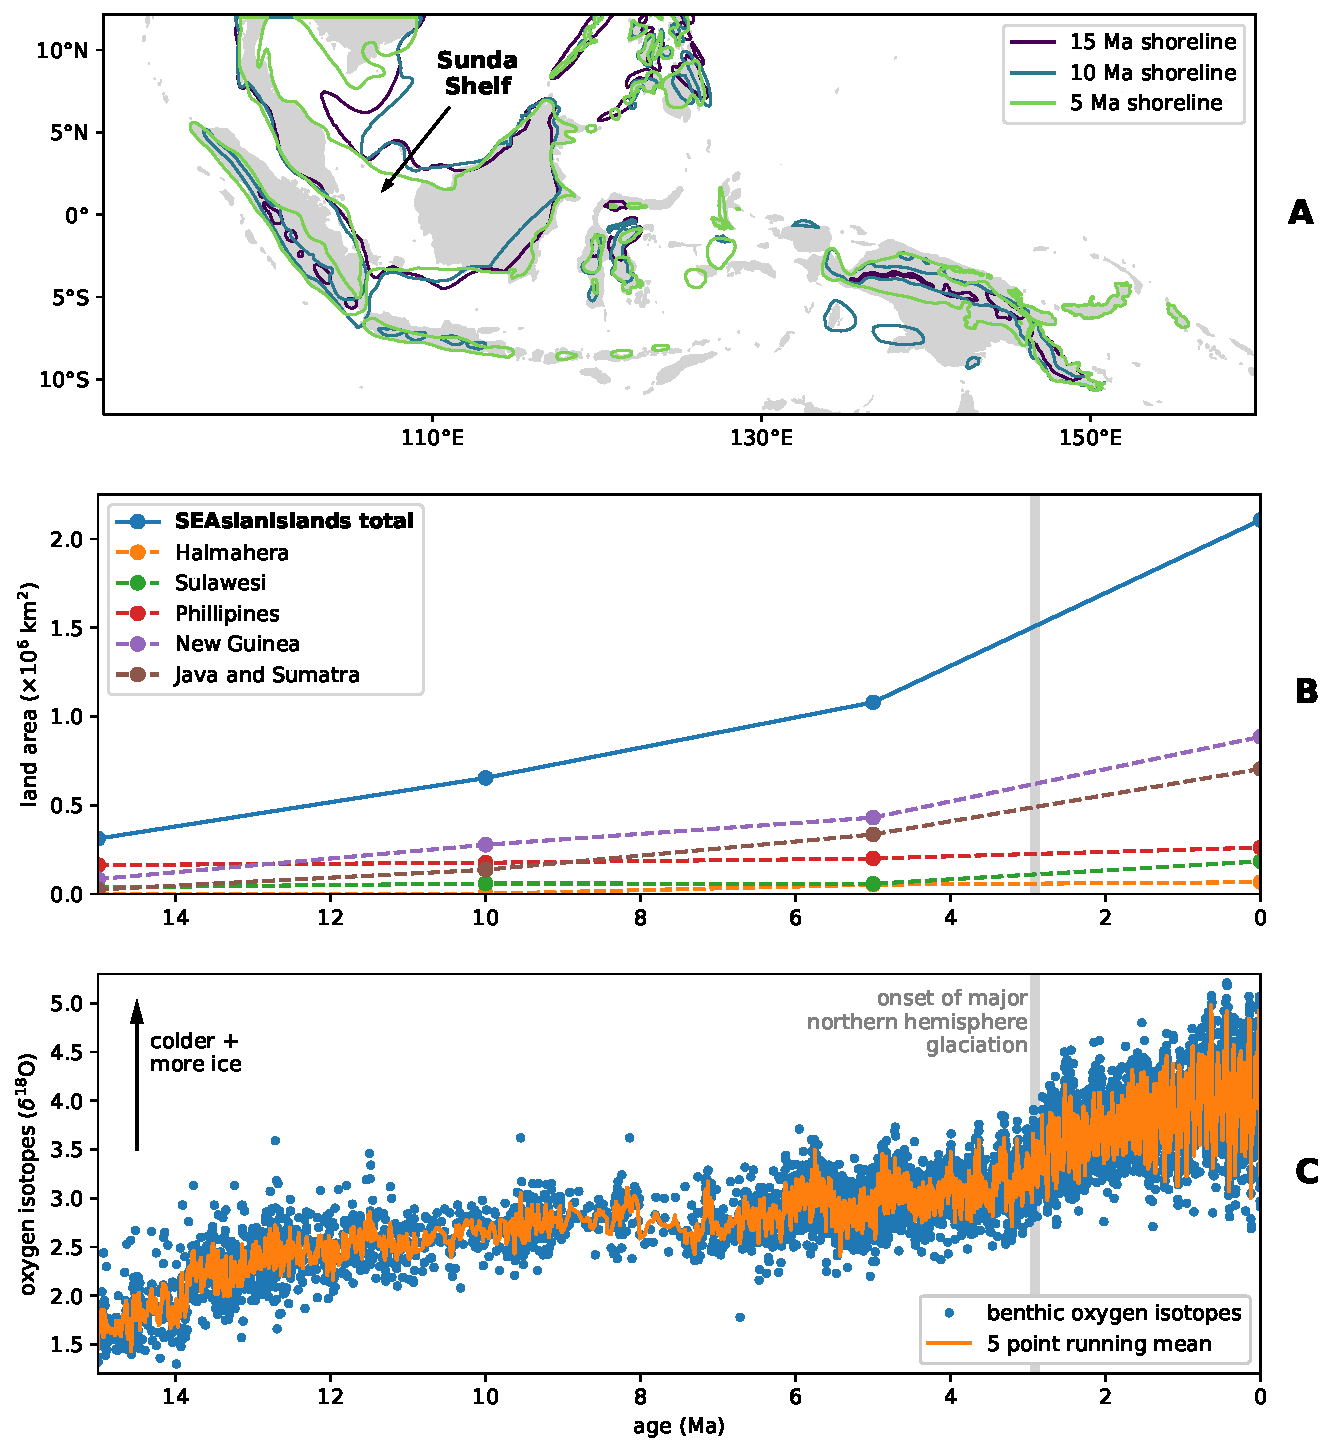
\includegraphics[width=0.9\textwidth]{Figures/shoreline_growth.pdf}
    \caption{The emergence of Indonesia and New Guinea (I\&NG) from the mid-Miocene to present in the region referred to in climate science literature as the Maritime Continent. Past shorelines are shown in A with associated area estimates summarized in B (where I\&NG refers to the sum of all the subdivided regions). A significant increase in area over the past 5 million years is coincident with cooling and the onset of Northern Hemisphere glaciation as reflected in the benthic oxygen isotope record \cite{Zachos2008a} in C.}
    \label{fig:shoreline_growth}
\end{figure}

\begin{figure}[h!]
    \centering
    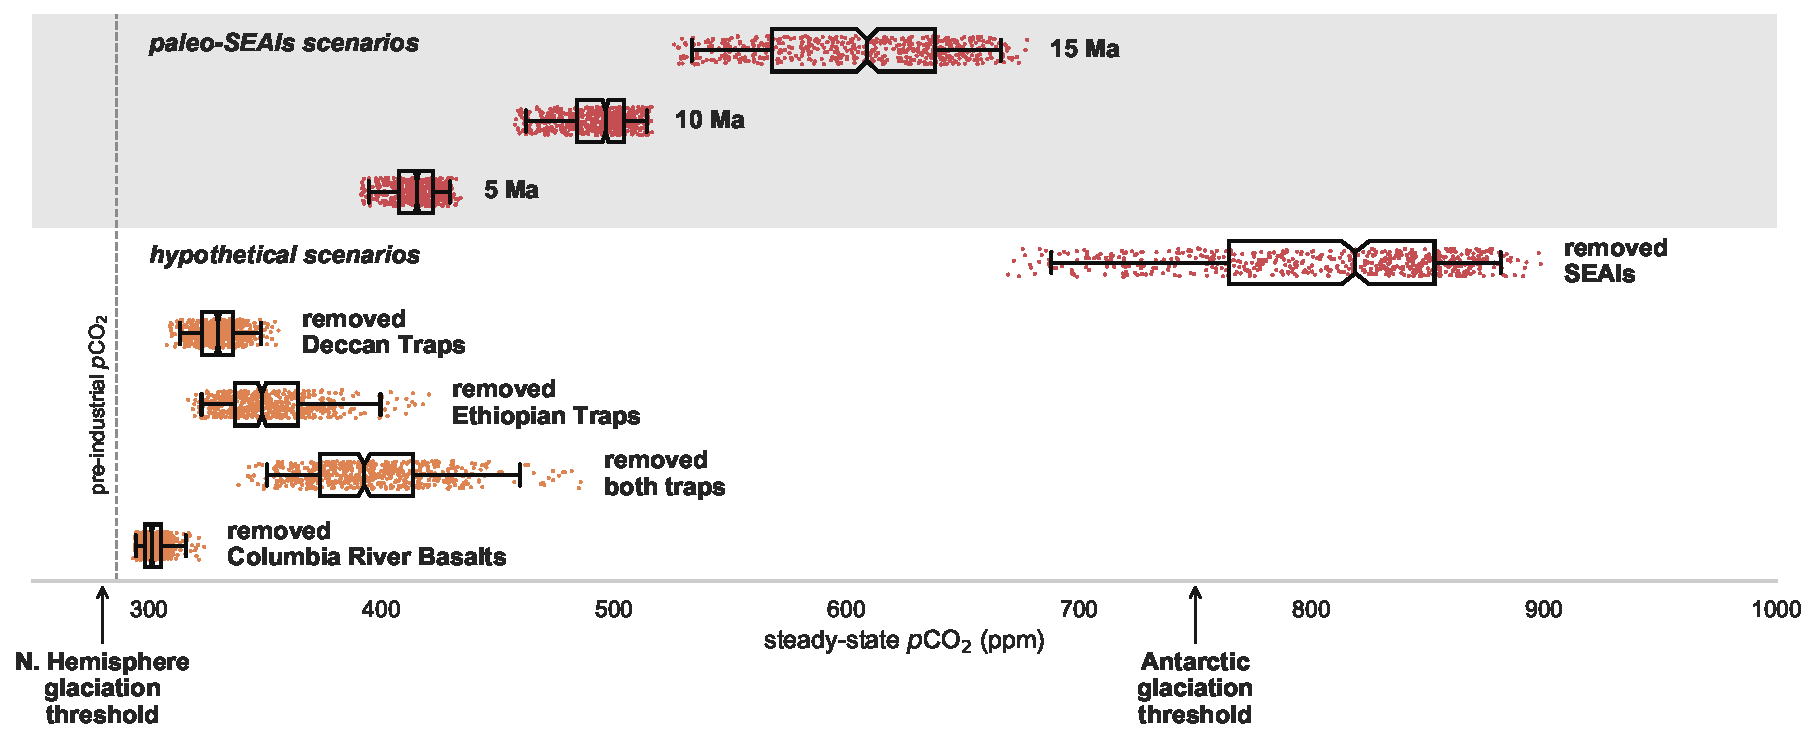
\includegraphics[width=1\textwidth]{Figures/scenario_pCO2.pdf}
    \caption{Steady-state \pCOtwo estimates from GEOCLIM for the various scenarios discussed in the text. For each of the seven scenarios, each point represents an estimate from one of the 3,339 unique parameter combinations that resulted in reasonable total global \COtwo consumption and most closely matched \COtwo consumption estimated from watershed data (see SI). The box encloses the middle 50\% of the \pCOtwo estimates (i.e. the interquartile range), and the notch represents the median with its 95\% confidence interval. The whiskers extend to 1.5$\times$ the interquartile range, or to the minimum/maximum of the estimates if no estimates are below/above this range.}
    \label{fig:scenario_pCO2}
\end{figure}

\clearpage
\newpage
\footnotesize

\singlespacing

\bibliographystyle{nature}
\bibliography{References}

\end{document}